\documentclass[10pt]{article}
\usepackage[export]{adjustbox}
\usepackage{graphicx}
\begin{document}
	
	
\begin{tabbing}
	\hspace{1.75in}
	\LARGE{\bf Nagesh K} % Print the main header
\end{tabbing}
%------------------------------------------------

\makebox[\linewidth]{\rule{18cm}{0.4pt}}
\vspace{.05 in} \\
\noindent\hspace{-1 in}
\begin{tabular}{@{}p{3.25in}p{3in}}
	
	No.214/1, 7\textsuperscript{th} Cross,             & {Phone:}  9739530539 \\
	Kurubarahalli, 
	& {E-mail:}  nagu1997@gmail.com\\
	Bangalore - 560086  
\end{tabular}

	\begin{figure}[h]
		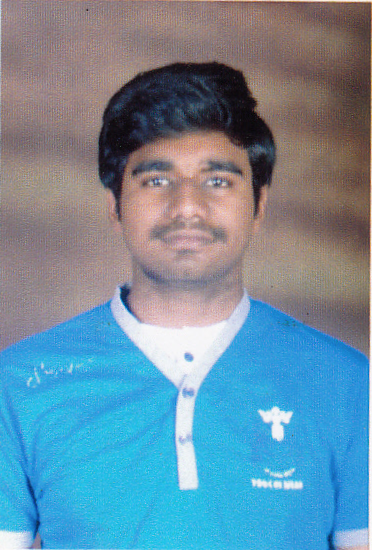
\includegraphics[width=0.2\textwidth,right]{photo.png}
	\end{figure}
	
	
		\underline{\textbf{\Large{OBJECTIVE}}}\\
		
		To constantly upgrade my knowledge and skills and make a difference in whatever I do.\\
		
%	\hfill\\	
	\underline{\textbf{\Large{EDUCATION}}}
	\vspace{-0.5cm}
	
	\hfill\\
	\hfill\\
	%\noindent\flushleft%\vspace{.3in}
	%\hspace{-0.9in}
	\begin{tabular}{|c|c|c|c|c|}
		\hline
		\bf Degree & \bf College/School & \bf University & \bf Passing Year & \bf  Percentage \\
		\hline
		Bachelor of & RV College of & VTU & 2019 & 9.03\\
		Engineering &  Engineering &  & (Pursuing) & (3 sems)\\
		\hline
		Pre-& S Nijalingappa & - & 2015 & 96\\
		University & PU College & & &\\
		\hline
		Secondary & Twinklers & - & 2013 & 96 \\
		School & High School & & & \\
		\hline
	\end{tabular}
	
	\vspace{0.5cm}	
	\underline{\textbf{\Large{PROJECTS}}}
	\begin{enumerate}
		\item{\underline{\textbf{\large{Robotic Arm:}}} This project aims at providing a remotely controlled substitute for the arm. This   also aims at industrial automation.}
		\item{\underline{\textbf{\large{Trailblazer:}}} Organized by NIT Surathkal.This project aims at developing a bot capable decoding realtime data . This uses the concept of line follower to follow the line while decoding the information on the ground. The information is in the form of black patches which is recognized using an IR sensor..}
		\item{\underline{\textbf{\large{e-Yantra:}}} Organized by IIT Bombay. This project aims at tackling one of the basic challenges faced by the mars rover i.e. crossing the crater. This project uses concept of image processing to identify the obstacles, cavities etc. An efficient path is planned based on this information which is sent to the rover.}
		\item{\underline{\textbf{\large{LED Cube:}}} This project aims at developing a multipurpose cube for both education and entertainment purpose. It is 4X4X4 LED matrix replicating a Rubiks cube.}
		\item{\underline{\textbf{\large{Line Follower:}}} This project aims at developing a model to replace the present rail system in industries. The prototype uses IR LEDs to recognize the white line.'}
		\item{\underline{\textbf{\large{Snake Game:}}} This project aims at developing a game. It uses 64X64 graphical LCD for display. 8051 Microcontroller is used to interface the LCD and to accept the user inputs, based on which the snake is controlled.'}
	\end{enumerate}
	
	\hfill
	%\vspace{1cm}
	
		\underline{\textbf{\Large{TRAINING AND INTERNSHIP}}}
		\begin{itemize}
			\item{Conducted a 'Basic Robotics Workshop' for class 12 students.}
			\item{Attended a Workshop on "PCB Design".}
		\end{itemize}
		
		\hfill 
		
		
		
		%\vspace{1cm}
		
		\underline{\textbf{\Large{RESEARCH PUBLICATION}}}
		\begin{itemize}
			
		\end{itemize}
		
		\hfill 
		\hfill
	
			\underline{\textbf{\Large{SOFT SKILLS}}}
			\begin{enumerate}
				\item{Hard working, dedicated and punctual}
				\item{Team work and responsibility}
				\item{leadership qualities} 
				
			\end{enumerate}
			
			\hfill
			
		\underline{\textbf{\Large{EXTRACURRICULAR ACTIVITIES}}}
		\begin{itemize}
			\item{Volunteered as a student mentor at the 'The Akshay Patra Foundation', an NGO in Bangalore.}
			\item{Been a 'Head Boy' in my school.}
			
		\end{itemize}
		
		\hfill
		
			\underline{\textbf{\Large{CO-CURRICULAR ACTIVITIES}}}
			\begin{enumerate}
				\item{Participated in inter-college quiz contests.}
				\item{Organized few inter-college competitions.}
				\item{Part of acting club in RV.}
				\\	
				\\				
				
			\end{enumerate}
			
			\underline{\textbf{\Large{ACHIEVEMENTS}}}
			\begin{itemize}
				\item{Participated and won \textbf{1\textsuperscript{st}
					place in Engineer 2016,“Trailblazer”} event organized
					by NIT-Surathkal.}
				\item{Participated and won \textbf{4\textsuperscript{th}
					place in e-Yantra 2017,“Cross the Crater”} theme
					organized by IIT-Bombay.}
				
			\end{itemize}
			
			
			\hfill
			
				\underline{\textbf{\Large{Personal details}}}
				
				\parbox{1.5\textwidth}{ % First block
					\begin{tabbing} % Enables tabbing
						\hspace{3cm} \= \hspace{4cm} \= \kill % Spacing within the block
						{ Father's Name} \> Keshava Kumar A\\
						{ Mother's Name} \> Asha P S\\
						{ Sex} \> Male\\
						{ Date of Birth} \> 23$^{rd}$ Jan 1998  \\ 
						{ Nationality} \> Indian \\
						{ Marital Status} \> Single\\
				\end{tabbing}}
				\\
				\hfill
				
				\underline{\textbf{\Large{Reference}}} \\
				\hfill
				
					\underline{\textbf{\Large{Declaration}}} \\
					
					I hereby declare that the above information is true to the best of
					my knowledge
					
					\hfill\\
					
					\underline{\textbf{\large{Date:}}}  {\em\today}
	
\end{document}